 % - IPC Functionality
 %  - Minimum required per subnet
 %    - Withdrawal/Deposits Interfaces
 %    - Other Operations? (Propagate?)
 %  - Enhancements
 %    - Checkpointing interfaces
 %    - Propagate
 %    - Reporting/Slashing interfaces
 %    - Atomic execution/swap, IBC-like bridges
 %  - Future stuff (google docs?)
 %    - Withdrawal at ancestor (skip parent(s)) (with timeout) etc.
\section{IPC functionality}
\label{sec:functionality}

IPC exposes the following functionalities:
\begin{itemize}
    \item Creating child subnets.
    \item Removing child subnets.
    \item Depositing coins from an account in a subnet to an account in its child.
    \item Withdrawing coins from an account in a subnet to an account in its parent.
    \item Checkpointing - including a checkpoint of a subnet's replicated state in the replicated state of its parent.
    \item Propagating cross-net-transactions - invoking smart contracts in a subnet through changes in the replicated state of another subnet.
\end{itemize}
In the following, we describe each functionality in detail.

\subsection{Creating a child subnet}

Any user of a subnet $P$ can create a new subnet $P/C$ by submitting a transaction $P.\gw.CreateChild(P/C, params)$.
This results in the creation of a new subnet actor $\sa_C$ in $P$ governing the subnet $P/C$.
The \emph{params} value describes all the subnet-specific parameters required to initialize the state of $P.\sa_C$,
such as the initial membership data, the consensus protocol to use, etc.

\subsection{Deposits}
\label{sec:deposit}

\del{
\arp{Consider need to pause/remedy subnet after deposit (e.g. collateral not enough with new supply). IPC agent should check in that case}\guy{Does this comment belong here or somewhere else?}\\
}

A deposit is a transfer of funds (of some amount \fil) from \replace{a user $\user$ account in the parent subnet to $\user$'s account}{an account \src in the parent subnet $P$ to an account \dest} in the child subnet $P/C$.
\replace{We assume that $\user$ is a participant running a parent replica, a child replica, and an \ipc agent%
\footnote{If $\user$ does not run these processes, then it contacts a trusted participant that does and that performs the deposit on $\user$'s behalf.}
}{We assume that the owner of \src is either running their own IPC Agent to perform the necessary operations described below, or uses another trusted IPC agent to act on their behalf}.
The deposit is performed as follows:
\begin{enumerate}
    \item The \replace{local \ipc agent}{owner of \src} submits \replace{to the parent \smr replica the corresponding (properly signed)}{a} transaction
    $\tx=\textit{P.\sa.Deposit}\left(\src, \fil, \dest \right)$.
    \item The parent subnet orders and executes the \emph{Deposit} transaction (provided $\src$ has enough funds) by transferring \fil from \replace{$\user$'s parent account}{\src} to the \sa (concretely, to $\dest$ account representation within the \sa). This effectively locks the funds within the \sa \dapp, until the \sa \dapp transfers it back to $\src$ during a withdrawal (see \Cref{sec:withdraw}).
    \item When the parent's replicated state that includes \replace{the transaction}{\emph{tx}} becomes final (for some SMR-system-specific definition of finality),
    \replace{the local parent replica notifies the local \ipc agent, potentially attaching a proof of finality of \prf to the notification.}{
    The \ipc agent constructs a $\pof(tx)$\footnote{The exact content of \prf for the transaction \tx depends on the implementations of the SMR systems. It might contain, for example, a quorum of replica signatures, a Merkle proof of inclusion, or even be empty.}
    }
    \item xThe IPC Agent submits a transaction $\tx' = \textit{P/C.Deposited}(\fil, \dest, \pof)$ to the child SMR system.
    \item Upon ordering $\tx'$, the replicated logic of the child SMR system mints \fil new coins and adds them to $\dest$.
\end{enumerate}

\replace{We show in \Cref{fig:deposit} t}{T}he events being produced and consumed by the deposit functionality and in Algorithm~\ref{alg:deposit} the pseudocode per component to implement the functionality.

% \begin{figure}[h]
%      \centering
%      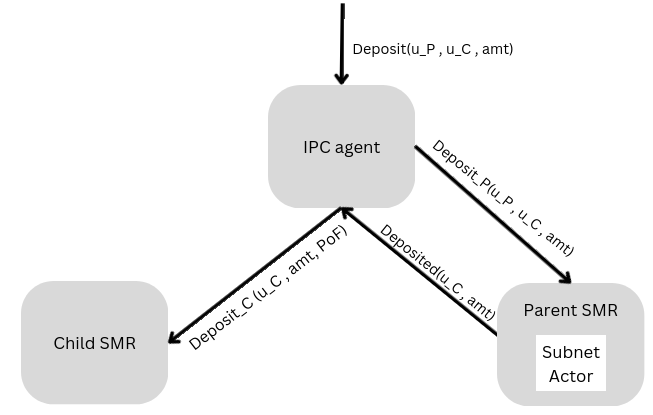
\includegraphics[width=\textwidth]{deposit}
%      \caption{Events produced and consumed during a deposit.}
%      \label{fig:deposit}
% \end{figure}
 

\begin{algorithm}[H]
\footnotesize
\caption{Deposit operation}\label{alg:deposit}
  \DontPrintSemicolon
  \SetKwFunction{FMain}{Global}
  \SetKwProg{Pn}{Function}{:}{\KwRet}
  \SetKwInOut{Input}{input}
  \SetKwProg{Component}{$\blacktriangleright$ \bf}{:}{\KwRet}
  \SetKwFor{UponKW}{upon}{do}{fintq}

   \Component{\replace{IPC agent}{Owner of \src}}{
        submit $\tx=\textit{P.\sa.Deposit}\left( \src, \fil, \dest \right)$ to parent subnet\;
  }
   \Component{P.\sa.Deposit(\src, amt, \dest)}{
    move $\fil$ from \src to P.\sa.\textit{accounts}.\dest  \tcp*[r]{"lock" at parent}
  }
  \Component{IPC agent}{
    \UponKW{tx = P.\sa.Deposit final at parent}{
        create \prf that \tx is final at parent subnet \tcp*[r]{see \cref{sec:finality}}
        submit \textit{P/C.\gw.Deposited(amt, \dest, \pof)}
     }
  }
  \Component{\replace{Child \smr replica}{P/C.\gw.Deposited(amt, \dest, \pof)}}{
%    \UponKW{\texttt{Deposited}}{
        \replace{assert \gw.\verifyPfinal{\tx}{\prf}}{verify(\pof)}\;
        increase \dest account by \fil
%     }
  }
\end{algorithm}

\subsection{Withdrawals}
\label{sec:withdraw}

A withdrawal is a transfer of funds from \replace{a user $\user$ account in the child subnet to $\user$'s account in the parent subnet. We assume that $\user$ is a participant running a parent replica, a child replica and an \ipc agent.}{an account \src in the child subnet $P/C$ to an account \dest in the parent subnet $P$}.
The \replace{withdraw}{\emph{Withdraw}} is performed \replace{as follows}{analogously to the \emph{Deposit}, but starting at the child subnet $P/C$}:
\begin{enumerate}
  \item \replace{$\user$ triggers the}{The owner of \src submits a transaction \emph{tx =}} $\textit{P/C.\gw.Withdraw}(\src, \fil, \dest)$.
    \item The child \replace{SMR system}{subnet} orders and executes the \emph{Withdraw} transaction, burning $\fil$ funds in $\src$ (provided $\src$ has enough funds).
    \item When the child's replicated state that includes the transaction becomes final (for some SMR-system-specific definition of finality that has been defined in the SA), the \replace{local child replica notifies the local \ipc agent, potentially attaching a proof \prf that this state is final}{\ipc agent constructs a corresponding \pof and submits a transaction \textit{\tx' = P.\sa.Withdrawn(\fil, \dest, \pof)} to the parent subnet}.
    \item Upon ordering $\tx'$, \replace{the replicated logic of the parent SMR system updates the state of the \sa transferring the funds}{\emph{P.\sa.Withdrawn(amt, \dest, \pof)} verifies the \pof and transfers \emph{amt}} from \sa (concretely, to $\src$ account representation within the \sa) to $\dest$ within the parent subnet.
\end{enumerate}

 % \begin{figure}[h]
 %     \centering
 %     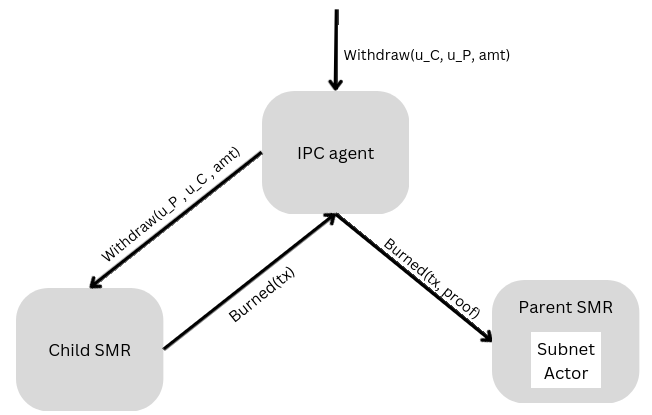
\includegraphics[width=\textwidth]{withdrawal}
 %     \caption{Events produced and consumed during a withdrawal.}
 %     \label{fig:withdrawal}
 % \end{figure}
\begin{algorithm}[H]
\footnotesize
\caption{Withdraw operation}\label{alg:withdraw}
  \DontPrintSemicolon
  \SetKwFunction{FMain}{Global}
  \SetKwProg{Pn}{Function}{:}{\KwRet}
  \SetKwInOut{Input}{input}
  \SetKwProg{Component}{$\blacktriangleright$ \bf}{:}{\KwRet}
  \SetKwFor{UponKW}{upon}{do}{fintq}
  % \Input{user~$\user$, amount~$\fil$, transaction \txnf}
   \Component{\replace{IPC agent}{owner of \src}}{
        submit $\tx=\textit{P/C.\gw.Withdraw}(\src, \fil, \dest)$\;
  }
   %
   \Component{\replace{Child \smr replica}{\textit{P/C.\gw.Withdraw(\src, \fil, \dest)}}}{
   \replace{\UponKW{$\tx = \textit{Withdraw}(\src, \fil, \dest)$}{
    deduct $\fil$ from \src \tcp{"burns" \fil in child}
   }}{
    deduct $\fil$ from \src \tcp{"burns" \fil in child}
   }
  }
  \Component{IPC agent}{
    \UponKW{\replace{notification of \texttt{Burned}(\tx) from child \smr replica}{tx = P/C.\gw.Withdraw(\src, \fil, \dest)} final at child}{
        create \replace{\prf that \tx is final at child \smr}{$\pof(tx)$} \tcp*[r]{see \cref{sec:finality} for details}
        submit \replace{$\tx'=\texttt{Burned}\left(\tx, \prf \right)$  to parent \smr replica}{\textit{P.\sa.Withdrawn(amt, \dest, \pof)}}
     }
  }
  \Component{P.\sa.Withdrawn(amt, \dest, \pof)}{
    \replace{assert \sa.\verifyGfinal{\prf}{\tx}}{verify($\pof(tx')$)}\;
    move \fil coins from P.\sa to \dest \tcp{"unlocks" \textit{amt} for \dest}
  }
   
\end{algorithm}
\label{enhancedFunc}

\subsection{Checkpointing} 
A checkpoint contains a representation of the state of the child \replace{SMR system}{subnet} to be included in the parent \replace{SMR system}{subnet's replicated state}. A checkpoint can be triggered by predefined events (e.g.,  periodically after a number of state updates, triggered by a specific user or set of users, etc.).
A checkpoint is \replace{performed}{created} as follows:
\replace{
\begin{enumerate}
\item When the predefined checkpoint trigger is met (the IPC Agent, monitoring the child subnet's state, is configured with the checkpoint trigger), the IPC agent queries the parent's \sa.
\item If the participant is a validator according to \sa's state, then the IPC agent queries the child SMR replica for the child's state to be represented in this checkpoint. 
\item The IPC agent creates a \prf that this updated state of the child SMR system is final, possibly compressing its representation of the state. 
\item The IPC agent evaluates a function \ssc(sa, parent's state, etc.) and decides whether the participant submits the checkpoint. If the function returns true, then the IPC agent submits a transaction $\tx=\texttt{Checkpoint}\left(\textit{state}, \prf \right)$ to the parent SMR replica.
 \item Upon ordering $\tx$, the replicated logic of the parent SMR system updates the state of the SA according to the checkpoint state, if necessary.
\end{enumerate}
}{
\begin{enumerate}
    \item When the predefined checkpoint trigger is met (the IPC Agent, monitoring the child subnet's state, is configured with the checkpoint trigger),
    the IPC agent retrieves the corresponding checkpoint data (\emph{chkp}) from the child subnet, along with the proof of its finality (\emph{\pof}).
    \item \TODO{Here the IPC Agent should decide (based on rights and some possible reward) whether to submit the Checkpoint transaction.}
    \item The IPC agent submits a transaction \emph{tx = P.\sa.Checkpoint(chkp, \pof)}.
    \item The \emph{P.SA.Checkpoint(chkp, \pof)} invocation, after verifying the \emph{\pof}, includes \emph{chkp} in its state.
\end{enumerate}
}

% \TODO{Pseudocode}
% See commented algorithm

% \begin{figure}[h]
%      \centering
%      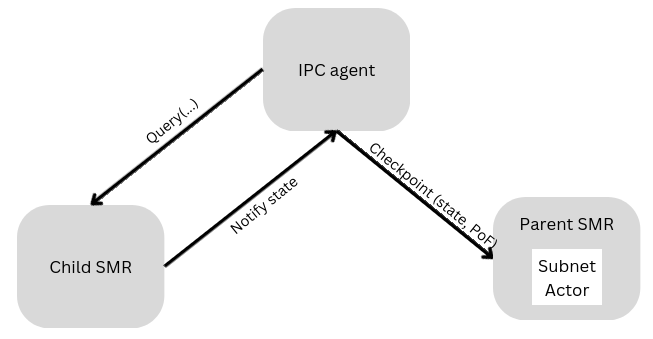
\includegraphics[width=\textwidth]{checkpoint.png}
%      \caption{Events produced and consumed by the checkpointing functionality.}
%      \label{fig:chkp}
%  \end{figure}

\begin{algorithm}[H]
\footnotesize
\caption{Checkpoint operation}\label{alg:checkpoint}
  \DontPrintSemicolon
  \SetKwFunction{FMain}{Global}
  \SetKwProg{Pn}{Function}{:}{\KwRet}
  \SetKwInOut{Input}{input}
  \SetKwProg{Component}{$\blacktriangleright$ \bf}{:}{\KwRet}
  \SetKwFor{UponKW}{upon}{do}{fintq}

  \Component{IPC agent}{
    \UponKW{Checkpoint condition in child}{
      $chkp = $ obtain state snapshot from child\;
      create $\pof(chkp)$\;
      submit $P.\sa.Checkpoint(chkp, \pof(chkp))$
    }
  }

  \Component{P.\sa.Checkpoint(chkp, \pof(chkp))}{
    verify($\pof(tx')$)\;
    save $chkp$ in the state\;
    \TODO{Expand on this. check if the checkpoint is the latest one and use a variable to store the latest checkpoint}
  }
   
\end{algorithm}

% OLD PSEUDOCODE
% \begin{algorithm}[H]
% \footnotesize
% \caption{Checkpoint operation\TODO{Update to new terminology}}\label{alg:down}
%   \DontPrintSemicolon
%   \SetKwFunction{FMain}{Global}
%   \SetKwProg{Pn}{Function}{:}{\KwRet}
%   \SetKwInOut{Input}{input}
%   \SetKwProg{Component}{$\blacktriangleright$ \bf}{:}{\KwRet}
%   \SetKwFor{UponKW}{upon}{do}{fintq}
%    \Component{IPC agent}{
%         \If{trigger for checkpoint}{
%             \textit{SA\_state} $\gets$ query parent for \sa's state\;
%             \If{\textit{Self} \textbf{in} SA\_state.validators}{
%                 \textit{state} $\gets$ query child for state\;
%                 \textit{cState} $\gets$ \textit{compressState}(\text{state},\textit{SA\_state.latestCheckpoint})\;
%                 create \prf that \textit{cState} is final at child\;
%             }
%             $\tx=\sa.\texttt{Checkpoint}\left(\textit{cState}, \prf \right)$ \;
%             \If{\textit{Self.}\ssc(tx, SA\_state, ...)}{
%                 submit $tx$ to parent \smr replica\;
%             }
%         }
%   }
%   \Component{parent \smr replica}{
%     \UponKW{$\tx=\sa.\texttt{Checkpoint}\left(\textit{cState}, \prf \right)$}{
%         assert \sa.\verifyGfinal{\textit{cState}}{\prf}\;
%         $\sa.\textit{latestCheckpoint.update}(\textit{cState})$
%      }
%   }
% \end{algorithm}

% The above pseudo code is intentionally abstract, with a number of implementation decisions not specified, such as the main function for creating and verifying a \prf, events that trigger the creation of a new checkpoint, the compression procedure with respect to the previous checkpoint, and the \ssc function to decide whether the participant submits or not a checkpoint. 

% The above pseudo code is highly abstract, with the main function of creating and verifying a \prf not specified. Moreover, other important aspects that are not covered include specific compression mechanisms for the checkpoint data, triggering checkpoints efficiently, and particular incentives for checkpoints creation and submission. \arp{we refer to reference implementation... later in this document we list others...}
% The function \ssc comprises two aspects of the checkpointing functionality from the perspective of participants. First, it controls access to submit checkpoints, as not all subnets will define the same policy to follow when deciding the participants that are allowed to submit checkpoints. Second, it contains the implications of submitting a checkpoint transaction (i.e. the cost involved in being the submitter). For example, if only one transaction is required by any participant but the cost of submitting the checkpoint is incurred on the submitter, then there is a risk of no participant actually submitting the checkpoint if they are strictly rational. An example on the other end might be requiring all participants to submit a transaction for the checkpoint to be finalized at the parent, but this approach affects performance. \arp{We analyze and suggest later in this document multiple mechanisms to ensure through incentives that at least one rational participant will always submit the checkpoint. }

\subsection{Propagating cross-net transactions}

Unlike a "standard" transaction issued and submitted to a subnet by a user,
a cross-net transaction is issued by the replicated logic of another subnet.
Cross-net transactions are a means of interaction between smart contracts located on different subnets.

Since those smart contracts themselves are not processes (but mere parts of a subnet's replicated state),
they cannot directly submit transactions to other subnets.
IPC therefore provides a mechanism to propagate these transactions between subnets using a ``\emph{postBox}'' and an IPC agent.
In a nutshell, if a smart contract's logic produces a transaction for a different subnet,
this transaction is saved the local Gateway Actor in a buffer that we call the \emph{postBox}.
The IPC agent, monitoring the postBox, then submits the transaction to the appropriate subnet.

Since, in general, we only rely on IPC Agents to be able to submit transactions to parents or children of a subnet whose state they observe,
the IPC agent only propagates the transaction to the parent or child, depending on which is closer in the IPC hierarchy to the ultimate destination subnet.
After such ``one hop``, the transaction is again placed in the postBox of the parent / child, and the process repeats until the transaction reaches its destination subnet.

The implementation of the Gateway Actor's \emph{Propagate} function is sketched in \Cref{alg:po}.

\TODO{Formalize subnet names and explain how the "\emph{src}" is built.}

% \guy{Edge case: a leaf subnet does not have a \sa and, therefore, no \postoffice. We can consider removing the \postoffice functionality from the \sa and to deploy it as an independent \dapp that will appear only once per subnet. In this case, it needs permissions to call \sa.\verifyGfinal{\tx}{\prf} function.}

\begin{algorithm}[H]
\footnotesize
\caption{Cross-net transaction propagation functionality}\label{alg:po}
  \DontPrintSemicolon
  \SetKwFunction{FPropagate}{propagate}
  \SetKwProg{Pn}{Function}{:}{\KwRet}
  \SetKwInOut{Input}{input}
  \SetKwProg{Component}{$\blacktriangleright$ \bf}{:}{\KwRet}
  \SetKwProg{Empty}{\bf}{:}{\KwRet}
  \SetKwFor{UponKW}{upon}{do}{fintq}
  \Component{\gw.Propagate($\tx, \src, \dest, \pof)$)}{
    verify(\tx.\pof)\;
    \Case{\dest = this subnet}{
        apply \tx
    }
    \Case{\dest requires going up the tree}{
       $postBox \leftarrow postBox \cup (\tx, S/\src, \dest)$\;
    }
    \Case{\dest requires going down the tree}{
        $postBox \leftarrow postBox \cup (\tx, \src/S, \dest)$\;
    }
  }
  \Component{IPC agent}{
    \UponKW{new entry (\tx, \src, \dest) in parent.\gw.postBox}{
        Create \pof proving that \tx' has indeed been added to the list fo cross-net transactions in the subnet\;
        submit \tx', augmented by \emph{\pof}
    }   
}
\end{algorithm}

\subsection{Slashing}
\arp{leave for later on with incentives and reconfiguration? it is hard to (meaningfully) talk about this without involving these concepts. Here a first attempt though:}
Slashing is a penalty imposed on provably malicious validators. When validators of a child subnet misbehave, other participants can report the misbehavior for these malicious validators to get punished (e.g. by losing a previously collateralized amount). Contrary to misbehaviors at a subnet with no parents, where misbehavers sucessfully perform their attack without escrow available, misbehaviors at the child can be resolved at the parent subnet, provided the misbehavers have not left the subnet.  For this reason, a slash focuses on notifying the parent subnet as soon as posible, in the hope to stop an attemped attack. In particular, a slash on provably malicious validators of a child subnet is performed as follows:
\begin{itemize}
    \item When the IPC agent of a correct participant identifies slashable misbehavior at subnet $P/C$ from a set $\mathcal{M}$ of malicious validators of subnet $P/C$, the IPC agent constructs a \textit{Proof of Misbehavior} (\pom). \item The IPC agent then submits transaction $tx_P=P.\sa.Slash(\mathcal{M}, \pom)$ at the parent and $tx_C=P/C.\gw.Slash.(\mathcal{M}, \pom)$ at the child.
    \item The parent subnet orders and executes $tx_P$. Once the parent's replicated state that includes $tx_P$ becomes final, the IPC agent constructs a $\pof(tx_P)$ and submits a transaction $\>\>\>\>\>\>$$tx'_P=P/C.\gw.Slashed(\mathcal{M}, \pom, \pof(tx_P))$
    \item When the child’s replicated state that includes $tx_C$ becomes final (for some SMR-system-specific definition of finality that has been defined in the SA), the IPC agent constructs a corresponding $\pof(tx_C)$ and submits a transaction $tx’_C = P.\sa.Slashed(\mathcal{M}, \pom, PoF)$ to the parent subnet.
    \item The parent subnet, upon ordering and executing either $tx_P$ or $tx_C'$, penalizes the misbehavers and updates the state of $\sa$. 
    \item The child subnet, upon ordering and executing either $tx_C$ or $tx_P'$, updates its state to reflect the penalization at the parent. \arp{This behavior at the child can later be updated to abort if it took place with $tx_C$ and in fact $tx_P'$ will never happen (i.e. attackers were faster and left subnet on time)} 
\end{itemize}
\begin{algorithm}[H] 
\arp{this alg must be updated, but RSs to converge on text above first}
\footnotesize
\caption{Slash Functionality}\label{alg:down}
  \DontPrintSemicolon
  \SetKwFunction{FMain}{Global}
  \SetKwProg{Pn}{Function}{:}{\KwRet}
  \SetKwInOut{Input}{input}
  \SetKwProg{Component}{$\blacktriangleright$ \bf}{:}{\KwRet}
  \SetKwFor{UponKW}{upon}{do}{fintq}
  \Input{-}
  \Component{Child SMR}{
     \UponKW{Proofs of fraud \pofs generated}{
       Notify \report to IPC agent
     }
  }
  \Component{IPC agent}{
    \UponKW{\report notified by child SMR}{
        Submit \slashop to parent SMR
    }
    \UponKW{\arp{State updated after slashing}}{
      \arp{Check child SMR rules are still satisfied, remedy/close otherwise?}
    }
  }
  \Component{Parent SMR}{
        \UponKW{\slashop submitted by IPC agent}{
         Update SA state slashing/excluding participants
         Notify SA update to IPC agent
        }
  }
\end{algorithm}


\subsection{Removing a child subnet}

A child subnet $P/C$ can be removed from its parent $P$ through a transaction invoking $P.\gw.RemoveChild(P/C)$.
\matej{We will later define a mechanism to determine who has the right to do this and when.}

% OLD PSEUDOCODE
% \begin{algorithm}[H]
% \footnotesize
% \caption{\postoffice Functionality}\label{alg:po}
%   \DontPrintSemicolon
%   \SetKwFunction{FPropagate}{propagate}
%   \SetKwProg{Pn}{Function}{:}{\KwRet}
%   \SetKwInOut{Input}{input}
%   \SetKwProg{Component}{$\blacktriangleright$ \bf}{:}{\KwRet}
%   \SetKwProg{Empty}{\bf}{:}{\KwRet}
%   \SetKwFor{UponKW}{upon}{do}{fintq}
%   \Input{$\tx = \langle \data, \src, \dest, \prf \rangle$}
%   \Component{\gw.\postoffice}{
%      \UponKW{\postoffice.\propagate(\tx) }{
%        \Case{\dest in current subnet}{
%             \postoffice.\propagate\textit{HERE}(\tx)
%        }
%        \Case{\dest requires going up the tree}{
%             \postoffice.\propagate\textit{UP}(\tx)
%        }
%        \Case{\dest requires going down the tree}{
%             \postoffice.\propagate\textit{DOWN}(\tx)
%        }
%      }
%      \UponKW{\postoffice.\propagate\textit{UP}(\tx) }{
%        \If{\src not from this subnet}{
%             assert \sa.\verifyGfinal{\tx}{\prf}\tcp*[r]{the \sa that corresponds to the child subnet from which \tx comes}
%        }
%        \src.\textit{append(\gw's subnet id)}\tcp*[r]{the i.d. of the current subnet}
%        emit event \gw.\postoffice.UP$\langle \data, \src, \dest \rangle$\;
%        % $\tx \gets \langle \data, \src, \dest \rangle$\;
%        notify agent on \gw.\postoffice.UP$\langle \data, \src, \dest \rangle$
%      }
%      \tcp{\propagate\textit{DOWN}(\tx) is analogous to \propagate\textit{UP}(\tx)}
%      \tcp{\propagate\textit{HERE}(\tx) is trivial}
%   }
%   % \Component{parent \smr process}{
%   %    \UponKW{event \postoffice.UP$\langle \data, \src, \dest \rangle$}{
%   %       $\tx \gets \langle \data, \src, \dest \rangle$\;
%   %       notify agent on \postoffice.UP(\tx)
%   %    }
%   % }
%   \Component{IPC agent}{
%     \UponKW{notification of \gw.\postoffice.UP$\langle \data, \src, \dest \rangle$ from child}{
%         $\tx' \gets$ \gw.\postoffice.UP$\langle \data, \src, \dest \rangle$\;
%         create \prf that \tx' is final at child \smr\;
%         $\tx_\textit{new}\gets\langle \tx', \prf \rangle$\;
%         submit \gw.\postoffice.\propagate($\tx_\textit{new}$) to parent \smr
%     }   
% }
% \end{algorithm}
% \subsection{Atomic Execution}
% TODO
